\documentclass[11pt]{article}
\usepackage[utf8]{inputenc}	% Para caracteres en español
\usepackage{amsmath,amsthm,amsfonts,amssymb,amscd}
\usepackage{multirow,booktabs}
\usepackage[table]{xcolor}
\usepackage{fullpage}
\usepackage{lastpage}
\usepackage{enumitem}
\usepackage{fancyhdr}
\usepackage{mathrsfs}
\usepackage{wrapfig}
\usepackage{setspace}
\usepackage{calc}
\usepackage{multicol}
\usepackage{cancel}
\usepackage{currency}
\DefineCurrency{GBP}{name={pound},plural={pounds},iso={GBP},kind=iso,symbol={\£}}
\usepackage[retainorgcmds]{IEEEtrantools}
\usepackage[margin=3cm]{geometry}
\newlength{\tabcont}
\setlength{\parindent}{0.0in}
\setlength{\parskip}{0.05in}
\usepackage{empheq}
\usepackage{framed}
\usepackage[most]{tcolorbox}
\usepackage{mdframed}
\usepackage{soul}
\usepackage{setspace}
\usepackage{hyperref}
\usepackage{pgfkeys}
\usepackage{subcaption}
\usepackage{tikz, pgfplots}
\usetikzlibrary{positioning}
\usepackage{float}

\newcommand\indep{\protect\mathpalette{\protect\independenT}{\perp}}
\def\independenT#1#2{\mathrel{\rlap{$#1#2$}\mkern2mu{#1#2}}}


\colorlet{shadecolor}{orange!15}
\parindent 0in
\parskip 12pt
\geometry{margin=1in, headsep=0.25in}

\theoremstyle{definition}
%\newtheorem*{note}{Note}

\newtheoremstyle{mystyle}{}{}{}{}{\sffamily\bfseries}{.}{ }{}
\newtheoremstyle{cstyle}{}{}{}{}{\sffamily\bfseries}{.}{ }{\thmnote{#3}}
\makeatletter
\renewenvironment{proof}[1][\proofname] {\par\pushQED{\qed}{\normalfont\sffamily\bfseries\topsep6\p@\@plus6\p@\relax #1\@addpunct{.} }}{\popQED\endtrivlist\@endpefalse}
\makeatother

\theoremstyle{mystyle}{\newtheorem{definition}{Definition}[section]}
\theoremstyle{mystyle}{\newtheorem*{note}{Note}}
\theoremstyle{mystyle}{\newtheorem*{example}{Example}}
\theoremstyle{mystyle}{\newtheorem*{procedure}{Procedure}}
\theoremstyle{mystyle}{\newtheorem{algo}{Algorithm}}

\tcolorboxenvironment{example}{boxrule=0pt,boxsep=0pt,blanker,borderline west={2pt}{0pt}{black},left=8pt,right=8pt,sharp corners,before skip=10pt,after skip=10pt,breakable}
\tcolorboxenvironment{definition}{boxrule=0pt,boxsep=0pt,colback={red!10},left=8pt,right=8pt,enhanced jigsaw, borderline west={2pt}{0pt}{red},sharp corners,before skip=10pt,after skip=10pt,breakable}
\tcolorboxenvironment{note}{boxrule=0pt,boxsep=0pt,blanker,borderline west={2pt}{0pt}{green},left=8pt,right=8pt,before skip=10pt,after skip=10pt,breakable}
\tcolorboxenvironment{procedure}{boxrule=0pt,boxsep=0pt,colback={blue!10},left=8pt,right=8pt,enhanced jigsaw, borderline west={2pt}{0pt}{blue},sharp corners,before skip=10pt,after skip=10pt,breakable}
\tcolorboxenvironment{proof}{boxrule=0pt,boxsep=0pt,blanker,borderline west={2pt}{0pt}{pink!80!white},left=8pt,right=8pt,sharp corners,before skip=10pt,after skip=10pt,breakable}

\tcolorboxenvironment{algo}{boxrule=0pt,boxsep=0pt,colback={black!10},left=8pt,right=8pt,enhanced jigsaw, borderline west={2pt}{0pt}{black},sharp corners,before skip=10pt,after skip=10pt,breakable}

\definecolor{codeblue}{rgb}{0.29296875, 0.51953125, 0.68359375}
\definecolor{codegreen}{rgb}{0.47265625, 0.62890625, 0.40234375}
\definecolor{codegray}{rgb}{0.95703125, 0.95703125, 0.95703125}
\definecolor{codecrimson}{rgb}{0.87109375,0.3984375,0.3984375}

\definecolor{contcol1}{rgb}{0.55, 0.71, 0.0}
\definecolor{contcol2}{rgb}{0.0, 0.5, 0.69}
\setcounter{tocdepth}{2}


% \verywidehat
{
\newcommand\reallywidehat[1]{%
\savestack{\tmpbox}{\stretchto{%
  \scaleto{%
    \scalerel*[\widthof{\ensuremath{#1}}]{\kern-.6pt\bigwedge\kern-.6pt}%
    {\rule[-\textheight/2]{1ex}{\textheight}}%WIDTH-LIMITED BIG WEDGE
  }{\textheight}% 
}{0.5ex}}%
\stackon[1pt]{#1}{\tmpbox}%
}}

%
% Title Page
%
\renewcommand{\part}[1]{\textbf{\large Part \Alph{partCounter}}\stepcounter{partCounter}\\}
\newcommand{\alg}[1]{\textsc{\bfseries \footnotesize #1}}
\newcommand{\deriv}[1]{\frac{\mathrm{d}}{\mathrm{d}x} (#1)}
\newcommand{\pderiv}[2]{\frac{\partial}{\partial #1} (#2)}
\newcommand{\dx}{\mathrm{d}x}
\newcommand{\solution}{\textbf{\large Solution}}


\newcommand{\E}{\mathbb{E}}
\newcommand{\Var}{\mathrm{Var}}
\newcommand{\Cov}{\mathrm{Cov}}
\newcommand{\Bias}{\mathrm{Bias}}

\definecolor{codeblue}{rgb}{0.29296875, 0.51953125, 0.68359375}
\definecolor{codegreen}{rgb}{0.47265625, 0.62890625, 0.40234375}
\definecolor{codegray}{rgb}{0.95703125, 0.95703125, 0.95703125}
\definecolor{codecrimson}{rgb}{0.87109375,0.3984375,0.3984375}

\newcommand*{\FormatDigit}[1]{\textcolor{blue}{#1}}
\lstdefinestyle{FormattedNumber}{%
    literate={0}{{\FormatDigit{0}}}{1}%
             {1}{{\FormatDigit{1}}}{1}%
             {2}{{\FormatDigit{2}}}{1}%
             {3}{{\FormatDigit{3}}}{1}%
             {4}{{\FormatDigit{4}}}{1}%
             {5}{{\FormatDigit{5}}}{1}%
             {6}{{\FormatDigit{6}}}{1}%
             {7}{{\FormatDigit{7}}}{1}%
             {8}{{\FormatDigit{8}}}{1}%
             {9}{{\FormatDigit{9}}}{1}%
             {.0}{{\FormatDigit{.0}}}{2}% Following is to ensure that only periods
             {.1}{{\FormatDigit{.1}}}{2}% followed by a digit are changed.
             {.2}{{\FormatDigit{.2}}}{2}%
             {.3}{{\FormatDigit{.3}}}{2}%
             {.4}{{\FormatDigit{.4}}}{2}%
             {.5}{{\FormatDigit{.5}}}{2}%
             {.6}{{\FormatDigit{.6}}}{2}%
             {.7}{{\FormatDigit{.7}}}{2}%
             {.8}{{\FormatDigit{.8}}}{2}%
             {.9}{{\FormatDigit{.9}}}{2}%
             %{,}{{\FormatDigit{,}}{1}% depends if you want the "," in color
             {\ }{{ }}{1}% handle the space
             ,
   basicstyle=\ttfamily,%  Optional to use this
}
\newcommand{\FormattedNumber}[1]{%
    \lstinline[style=FormattedNumber]{#1}%
}

\lstset{ 
  language=R,                     % the language of the code
  basicstyle=\ttfamily, % the size of the fonts that are used for the code
  numbers=left,                   % where to put the line-numbers
  numberstyle=\tiny\color{black},  % the style that is used for the line-numbers
  stepnumber=1,                   % the step between two line-numbers. If it is 1, each line
                                  % will be numbered
  numbersep=5pt,                  % how far the line-numbers are from the code
  backgroundcolor=\color{codegray},  % choose the background color. You must add \usepackage{color}
  showspaces=false,               % show spaces adding particular underscores
  showstringspaces=false,         % underline spaces within strings
  showtabs=false,                 % show tabs within strings adding particular underscores
  frame=single,                   % adds a frame around the code
  rulecolor=\color{black},        % if not set, the frame-color may be changed on line-breaks within not-black text (e.g. commens (green here))
  tabsize=2,                      % sets default tabsize to 2 spaces
  captionpos=b,                   % sets the caption-position to bottom
  breaklines=true,                % sets automatic line breaking
  breakatwhitespace=false,        % sets if automatic breaks should only happen at whitespace
  keywordstyle=\color{codeblue},      % keyword style
  commentstyle=\color{codegreen},   % comment style
  stringstyle=\color{codecrimson},      % string literal style
  xleftmargin = 0cm
} 

\newcommand\reallywidehat[1]{%
\savestack{\tmpbox}{\stretchto{%
  \scaleto{%
    \scalerel*[\widthof{\ensuremath{#1}}]{\kern-.6pt\bigwedge\kern-.6pt}%
    {\rule[-\textheight/2]{1ex}{\textheight}}%WIDTH-LIMITED BIG WEDGE
  }{\textheight}% 
}{0.5ex}}%
\stackon[1pt]{#1}{\tmpbox}%
}
%%%%%%%%%%%%%%%%%%%%%%%%%%%%%%%%%%%%%%%%%%%%%%%%%%%%%%%%%%%%%
\begin{document}
\title{Data Science for Economics}

\thispagestyle{empty}

\begin{center}
{\LARGE \bf Data Science for Economics}\\
{\large Archie Cannon}\\
\today
\end{center}
% use \begin{shaded} and \begin{note}

% Contents (all formatting here, other than colours)
{
\begin{tcolorbox}[title=Contents, fonttitle=\huge\sffamily\bfseries\selectfont,interior style={left color=contcol1!50!white,right color=contcol2!50!white},frame style={left color=contcol1!80!white,right color=contcol2!80!white},coltitle=black,top=2mm,bottom=2mm,left=2mm,right=2mm,drop fuzzy shadow,enhanced,breakable]
\makeatletter
\@starttoc{toc}
\makeatother
\end{tcolorbox}}

\newpage

\section{Regression}

We want to predict the response $y$ from inputs $\mathbf{x} = (1, x_1, x_2, x_3, \ldots, x_p)$. We can do this by modelling the \hl{conditional mean of $y$ conditional on $\mathbf{x}$}

\section{Cross Validation}

\section{Regularisation}

\subsection{PCR}
We talk about PCA in more detail in Section \ref{sec:PCA}

PCR offers a prediction technique and reduces the risk of overfitting through dimension reduction. We have found the principal components through PCA, we could use those components for regression. 

\section{Classification}

\newpage

\section{Tree-Based Methods}

Tree-based methods are simple and useful for interpretation but are usually not competitive with the best supervised learning approaches. We start to introduce techniques that make drastic improvements on the simple decision tree, like bagging and random forests.


\subsection{Decision Trees}

A logical system to map regressors to outcomes. They are \hl{hierarchical} meaning they use a series of ordered steps to come to a conclusion. We will be using data on baseball player salaries.

To illustrate, here is a decision tree:

\begin{figure}[h]
    \centering
    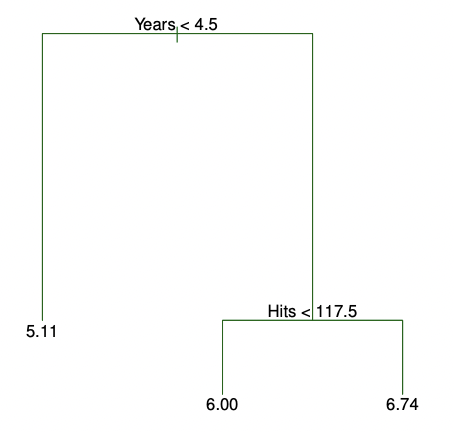
\includegraphics[width=6cm]{pic/decision tree.png}
    \caption{Decision Tree}
    \label{fig:decision tree}
\end{figure}

In this example, we are predicting player salaries and using the regressor \lstinline{hits} and \lstinline{years}. This decision tree can be visualised like so:

\begin{figure}[h]
    \centering
    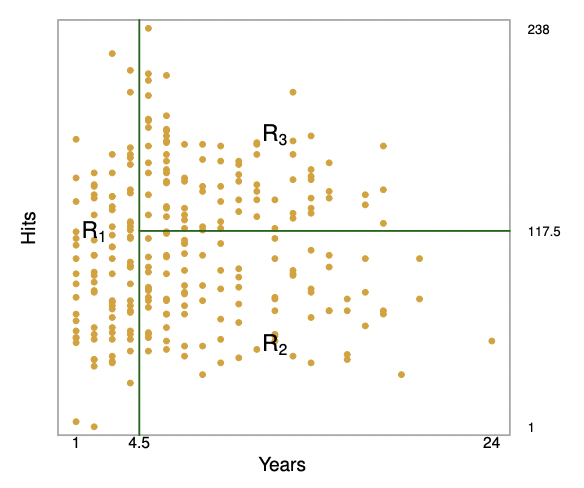
\includegraphics[width=6cm]{pic/decision tree parts.png}
    \caption{Decision Tree as Data}
    \label{fig:decision tree parts}
\end{figure}

At our \hl{primary node} we check whether the player has been in the league for less than 4.5 years. If so, we continue on the left. If the player has been in the league for over 4.5 years, then we continue to the next node on the right (hits $< 117.5$). The $R_1$ section in Figure \ref{fig:decision tree parts} corresponds to the left-most \hl{leaf} in Figure \ref{fig:decision tree}. $R_2$ corresponds to the middle leaf and $R_3$ corresponds to the right-most leaf. 

\begin{note}
    From both these Figures (\ref{fig:decision tree} \ref{fig:decision tree parts}) we can infer that, the average (log) salary for a player with less than 4.5 years of experience is 5.11; a player with more than 4.5 years of experience but less than 117.5 hits has an average (log) salary of 6.00; and a player with more than 4.5 years experience and more than 117.5 hits has an average (log) salary of 6.74.
\end{note}

\begin{shaded}
    \textbf{Terminology:}

    The tree splits input space $\mathbf{x} = \text{years, hits})$ in final nodes called \textbf{leafs}:

    \begin{itemize}
        \item $R_1 = \{\mathbf{x}|\text{years} < 4.5\}$
        \item $R_2 = \{\mathbf{x}|\text{years} \geq 4.5, \text{hits}<117.5\}$
        \item $R_3 = \{\mathbf{x}|\text{years} \geq 4.5, \text{hits}\geq 117.5\}$
    \end{itemize}

    Points on the tree where input space is split are called \textbf{internal nodes}. Segments connecting the nodes are \textbf{branches}.
\end{shaded}

So far we have an extremely simple tree, so we must grow it.

\subsubsection{Growing the Tree}

\begin{definition}
    Split $\mathbf{x}$-space in $J$ distinct, non-overlapping regions, $R_1, R_2, \ldots, R_J$. Suppose $\mathbf{x}_i \in R_j$; then the prediction for $y_i$ is $\hat{y} = \Bar{y} \equiv \frac{1}{n_j}\sum_{k:\mathbf{x}_k\in R_j} y_k$. Where $n_j$ is the number of observations that belong to $R_j$.

    \begin{note}
        This just means that for a given set of nodes (classifiers), our prediction will be the average of all the observations that fit said classifiers.
    \end{note}

    $R_1, R_2, \ldots, R_J$ are chosen to minimise the \textbf{loss function} (deviance).

    \begin{itemize}
        \item When $y$ is real: loss is the sum of squared errors (=regression deviance)

        \begin{equation*}
            \sum_{i=1}^n(y_i - \hat{y}_i)^2 = \sum_{j=1}^J \sum_{k:\mathbf{x}_k\in R_j}(y_k - \Bar{y})
        \end{equation*}

        \item When $y$ is binary: loss is the Gini impurity (or logit deviance)

        \begin{equation*}
            \sum_{i=1}^n \hat{y}_i(1-\hat{y}_i)^2 = \sum_{j=1}^J \sum_{k:\mathbf{x}_k\in R_j} \Bar{y}_j(1-\Bar{y}_j)^2
        \end{equation*}
    \end{itemize}
\end{definition}

Many ways to describe this algorithm:

The algorithm is \hl{greedy} as it makes the \textbf{locally} best choice at every step (similar to the forward step-wise regression). \hl{top-down} as it starts at the top of the tree. \hl{Recursive} as it solves the same problem in each step.

\subsubsection{Recursive Binary Splitting}

The node, $m$, is not split (leaf) it contributes cost:

\begin{equation*}
    \text{non-split node-}m \text{ cost} = \sum_{k:\mathbf{x}_k\in R_m}(y_k - \hat{y}R_m)^2
\end{equation*}

What the algorithm is doing is finding $x_j \in \{x_1, \ldots, x_p\}$ and cutoff $s$ to split $\mathbf{x}$-space into node-$m$ children

\begin{equation*}
    R_{left} = \{\mathbf{x}|x_j<s\}; \qquad R_{right} = \{\mathbf{x}|x_j \geq s\}
\end{equation*}

to minimise our cost function:

\begin{equation*}
    \text{split-node-}m \text{ cost} = \underbrace{\sum_{k:\mathbf{x}_k\in R_{left}}(y_k - \hat{y}R_{left})^2}_{\text{left cost}} + \underbrace{\sum_{k:\mathbf{x}_k\in R_{right}}(y_k - \hat{y}R_{right})^2}_{\text{right cost}}
\end{equation*}

So we are determining which parent node $m$ gives the maximum cost reduction by splitting, \hl{i.e. which regressor and cutoff reduces the cost function the most}. We keep doing this until a \textbf{convergence criterion} is met. This can be that each region (leaf) contains at least 3 observations. Or each split has to contribute a minimum decrease in deviance e.g. 0.001.


    
\begin{algo}

Tree creation:

\begin{center}

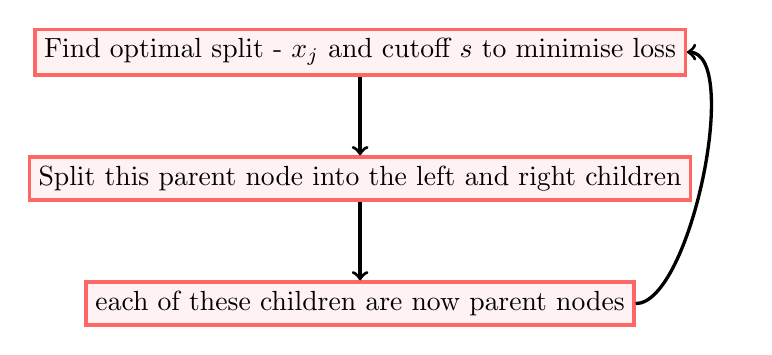
\begin{tikzpicture}[SIR/.style={rectangle, draw=red!60, fill=red!5, very thick, minimum size=5mm},]
%Nodes
\node[SIR] (1)     {Find optimal split - $x_j$ and cutoff $s$ to minimise loss};
\node[SIR] (2)[below=of 1] {Split this parent node into the left and right children};
\node[SIR] (3) [below=of 2] {each of these children are now parent nodes};

%Lines
\draw[->, very thick] (1.south)  to node[right] {} (2.north);
\draw[->, very thick] (2.south)  to node[right] {} (3.north);
\draw[->, very thick] (3.east) .. controls  +(right:7mm) and +(right:7mm)   .. (1.east);

\end{tikzpicture}
\end{center}
    
\end{algo}


This continues recursively until you reach a leaf node of some prespecified minimum size.

\subsubsection{Overfitting Our Tree}

\hl{When our tree is deep, it tends to be overfit}. The nonparametric nature of tree regressions means that it is very easy to overfit the data with an overgrown tree, leading to poor OOS predictions. An overgrown tree will be able to fit nonlinear mean and interaction effects without having to specify them (unlike linear regressions).

We have to prune the tree to constrain the flexibility and get better OOS predictions. We do this by:
\begin{itemize}
    \item construct a regularisation path of trees (from deep to shallow)
    \item Cross validate models along the path
\end{itemize}

\subsection{Cost Complexity Pruning}

A smaller tree with few splits (fewer regions) might lead to lower variance and better interpretation at the cost of a little bias. If we were to set the constraints very high (high minimum decrease in deviance) we may accidentally grow the tree too short and we miss a large reduction in RSS because of a small decrease before it. 

To avoid this we can grow a very complex and deep tree and then \textit{prune} it back in order to obtain a \hl{subtree}.

\begin{definition}
    \hl{Cost Complexity Pruning selects a sequence of subtrees} indexed by $\alpha>0$. Let $T_0$ be the complex tree; for each $\alpha>0$ find subtree $T_\alpha\subset T_0$ such that

    \begin{equation}
        \sum_{j=1}^{|T_\alpha}\sum_{k:\mathbf{x}_k\in R_k}(y_k - \Bar{y}_j)^2 + \alpha|T_\alpha|
    \end{equation}

    is minimised.

    \begin{note}
        $|T_\alpha|$ s the number of leaves on $T_\alpha$
    \end{note}

    Our \textbf{hyper-parameter} $\alpha$ penalises complexity (number of leaves); by varying $\alpha$ we obtain a regularisation path from complex to simple.

    \begin{note}
        $\alpha=0$ gives us the full tree. $\alpha\rightarrow\infty$ gives us a tingle leaf, $|T| = 1$.
    \end{note}

    We evaluate the OOS deviance for every tree on the path by cross-validation, then pick the subtree with the minimum OOS deviance.
\end{definition}



\subsubsection{Pros and Cons of Trees}

\begin{shaded}
    Pros:
    \begin{itemize}
        \item[+] Easy to explain (probably easier than regressions)
        \item[+] Can be argued that decision trees more closely mirror human decision making than regressions and classification methods
        \item[+] Easy to graph and interpret
        \item[+] Can easily handle qualitative regressors without the need for dummy variables.
    \end{itemize}

    Cons:
    \begin{itemize}
        \item[-] Do not tend to have the same predictive accuracy that regression models have 
        \item[-] Can be very unstable. Small changes in the data lead to drastic changes in the tree.
    \end{itemize}
\end{shaded}


\subsection{Ensemble Methods}


Trees can easily lead to overfitting. You \textit{can} do model selection by cross-validation, but the results are unstable and thus unreliable and impractical. Because there are no coefficients, we can't penalise the coefficients like we did before (we have now penalised the number of coefficients). 

Instead, we grow a \hl{forest} (= many trees) and regularise by \hl{bagging to obtain the random forest predictor}.



An ensemble method combines many simple models (aka "weak learners") to obtain a single powerful model. We look at both \hl{bagging and random forest} as ensemble methods that give better predictive power and stability.

\begin{note}
    We often see that when we use the ensemble approach there is usually a loss of interpretation in the final model.
\end{note}

\subsubsection{Bagging}

An overgrown tree is typically overfitted i.e. low bias and high variance. Bagging offers a way of reducing the variance of a tree based on the idea that \textbf{averaging reduces variance}.

\begin{definition}
    Bagging:

    Suppose we have $B$ training datasets so we could grow $B$ trees. Given inputs $\mathbf{x}$, we can make $B$ predictions $\hat{y}^b(\mathbf{x})$; averaging yields

    \begin{equation*}
        \hat{y}_{avg}(\mathbf{x}) = \dfrac{1}{B}\sum_{b=1}^B \hat{y}^b(\mathbf{x})
    \end{equation*}

    which is the \textbf{bagging predictor}. 
\end{definition}

Bagging is an average of i.i.d trees and the bagging predictor has lower variance than each individual tree. We do not have $B$ datasets, we only have 1 so we \hl{resample with replacement} to create $B$ datasets.

\begin{note}
    resampling with replacement means that an individual observation can be sampled multiple times in one dataset.
\end{note}
\subsubsection{Random Forests}

Random forest is a slightly modified bagging procedure. The splits in the fitted trees are chosen optimally across a random sample of inputs (meaning at on a specific tree, each node only has the choice of a few of the original regressors to make the split).

It is this random selection of predictors at each node that reduces the correlation between the trees grown at the different bootstrapped training samples. This decorrelation may induce some bias in the prediction, it also reduces the prediction variance and often improves the prediction accuracy.

\subsubsection{Out-Of-Bag Error}

We can estimate the the test MSE by cross validation but for bagging-based predictors there is an easier way: \textbf{out-of-bag error} (OOB error).

It can be shown that each bagged tree utilises only around two-thirds of the observations. The remaining one-third of the observations not used to fit a given bagged tree are referred to as the out-of-bag observations. We can predict the response for the $i$th observation using each of the trees in which that observation was OOB. This will yield around $B/3$ predictions which we can then average over (for regressions) or take majority vote (classification models).

\section{Unsupervised Learning}

So far, our main objective has been dimension reduction on big data  i.e. learn low dimensional summary stats necessary for good decisions from high dimensional input $\mathbf{x}$. And \hl{so far, this has all be supervised}, i.e. we have a target variable $y$ (regress target $y$ on high dimensional $\mathbf{x}$ ti get one dimensional $\hat{y} = \mathbf{x}^\prime\hat{\beta}$).

\hl{In unsupervised machine learning there is no target or outcome variable.} We still have a high dimensional input $\mathbf{x}$, and we still want dimension reduction. It is common to find partially labelled data and in this case we often use unsupervised learning to split the data into groups; then use the labelled data to predict.

\subsubsection{Mixture models}

Cluster analysis is used to collect similar observations into groups. Suppose data $(\mathbf{x}_i)_{i=1}^n$ where $\mathbf{x} = (x_1, x_2, \ldots, x_p)$ is a vector with $p$ characteristics. Clustering represents the data as output from a mixture distribution.

\paragraph{Mixture Distribution}: $\mathbf{x}_i$ is drawn from one of $K$ \textbf{mixture components} $p_k(\mathbf{x}), k = 1, 2, \ldots, K$. These mixture components are multivariate distributions of $\mathbf{x}$. 

The \textit{Guassian mixture model} where $p$ characterises $\mathbf{x}$ are i.i.d with variance $\sigma_k^2$ is a common clustering model;

\begin{equation}
    p_k(\mathbf{x}_i) = \dfrac{1}{(2\pi\sigma_k^2)^{p/2}}\exp\left[-\dfrac{\sum_{j=1}^p (x_{ij}-\mu_{kj})^2}{2\sigma_k^2}\right]
\end{equation}

With our unlabelled data we do not know which of $K$ components $\mathbf{x}_i$ is from. We only see the characteristics of the observations:

\begin{equation*}
    p(\mathbf{x}_i) = \pi_1 p_1(\mathbf{x}_i) + \pi_2 p_2 (\mathbf{x}_i) + \ldots + \pi_k p_k (\mathbf{x}_i)
\end{equation*}

where $\pi_k$ is the probability that $\mathbf{x}_i$ comes from the component $k$.

\subsection{Factorisation by K-Means}

We look at K-means as a way to model mixture models. This means the data comes from differing distributions and because of this it is important to group the data to match this.

K-means clustering is a way of grouping observations and it comes from a simple and intuitive maths problem.

\begin{definition}
    Let $C_1, C_2, \ldots, C_K$ denote sets containing the indices of the observations in each cluster. These sets satisfy

    \begin{enumerate}
        \item $C_1 \cup C_2 \cup \ldots \cup C_K = \{1, \ldots, n\}$. i.e. all observations are accounted for.

        \item $C_k \cap C_{k^\prime} = \varnothing \quad \forall k \neq k^\prime$. i.e. clusters do not overlap. No observation belongs to multiple clusters.
    \end{enumerate}
\end{definition}

\begin{note}
    With K-mean clustering, we specify a desired number of clusters $K$. 
\end{note}

\textbf{Good} clustering is one for which the \textit{within-cluster variation} is as small as possible. The within-cluster variation for cluster $C_k$ is a measure $W(C_k)$ of the amount by which the observations within the cluster differ from each other. Hence we want to solve this problem:

\begin{equation*}
    \underset{C_1, \ldots, C_K}{\min}\left\{\sum_{k=1}^K W(C_k)\right\}
\end{equation*}

We ant to group the observations into $K$ clusters such that the total within-cluster variation, summed over all $K$ clusters, is as small as possible. %This within-cluster variation can be calculated in many ways, but we use the \textit{squared Euclidean distance}:

\begin{algo}
    K-means:

    \begin{center}
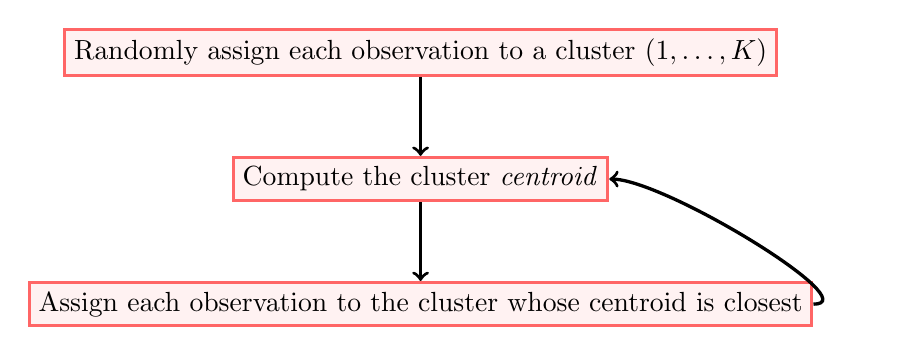
\begin{tikzpicture}[SIR/.style={rectangle, draw=red!60, fill=red!5, very thick, minimum size=5mm},]
%Nodes
\node[SIR] (1)     {Randomly assign each observation to a cluster ($1,\ldots, K)$};
\node[SIR] (2)[below=of 1] {Compute the cluster \textit{centroid}};
\node[SIR] (3) [below=of 2] {Assign each observation to the cluster whose centroid is closest};

%Lines
\draw[->, very thick] (1.south)  to node[right] {} (2.north);
\draw[->, very thick] (2.south)  to node[right] {} (3.north);
\draw[->, very thick] (3.east) .. controls  +(right:7mm) and +(right:7mm)   .. (2.east);

\end{tikzpicture}
\end{center}
\end{algo}

The cluster centroid is defined as:

\begin{equation*}
    \hat{\mu}_k = \Bar{x}_k = \dfrac{1}{n_k}\sum_{i:k_i = k}x_i
\end{equation*}
where $i: k_i = k$ are the $n_k$ observations with $k_i = k$.

In our example, $W(C_k)$ is the deviance:

\begin{equation*}
    W(C_k) = D_k = \sum_{j=1}^p (X_{ij} - \mu_{kj)^2}
\end{equation*}

Thus, our total deviance of $\{\mathbf{x}_i\}_{i=1}^n$ is 

\begin{equation*}
    D = \sum_{i=1}^n \sum_{k=1}^K 1_{k_i = k} \sum_{j=1}^p (x_{ij} - \mu_{kj})^2
\end{equation*}

\hl{But we do not know the cluster assignment $\{k_i\}_{i=1}^n$}. To minimise this deviance we have to estimate both the centroids and the assignment.

Objective: fit $\{\mu_k\}_{k=1}^K$ and $\{k_i\}_{i=1}^n$ to minimise the deviance

\begin{equation}
    \underset{\{\mu_k\}_{k=1}^K,\{k_i\}_{i=1}^n}{\min}\left(\sum_{i=1}^n \sum_{k=1}^K 1_{k_i = k} \underbrace{\left[\sum_{j=1}^p (x_{ij} - \mu_{kj})^2\right]}_{\text{within-cluster SS}}\right)
\end{equation}

where $k_i \in \{1,2,\ldots, K\}$ is the cluster assignment of observation $i$.

We can visualise this with the following figure

\begin{figure}[h]
    \centering
    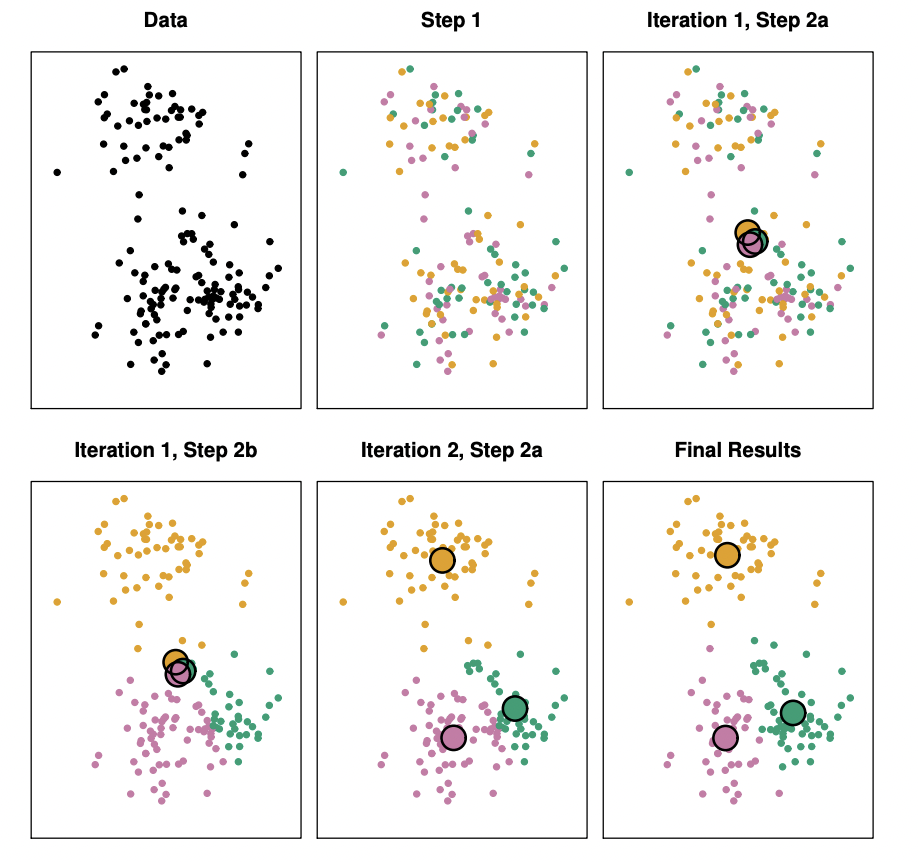
\includegraphics[width=13cm]{pic/k-means algo.png}
    \caption{Steps of the K-means algorithm}
    \label{fig:k-means algo}
\end{figure}

We repeat the algorithm until the cluster assignment no longer changes (convergence).

\subsubsection{Cons of K-means}

\begin{shaded}
    Drawbacks of the K-means algorithm:

    \begin{itemize}
        \item[-] How do we choose $K$. It is highly subjective.
        \item[-] Algorithm may converge on a local minima and not the global minima.
        \item[-] Local minima + initial randomisation means that multiple runs of the K-means algorithm on the same data may yield different results. 
    \end{itemize}

    To get around this we tend to do many runs with different initial random clusters and pick the run with the smallest sum-squared error.
\end{shaded}

It is common practice to report both the within- and between-cluster SS:

\begin{equation}
    \text{TSS} = \underbrace{\sum_{k=1}^K \sum_{i=1}^n 1 _{k_i = k}\left[\sum_{j=1}^p (x_{ij} - \mu_{kj})^2\right]}_{\text{\textbf{within}-cluster SS}} + \underbrace{\sum_{k=1}^K \sum_{i=1}^n 1 _{k_i = k}\left[\sum_{j=1}^p (\mu_{kj} - \mu_{j})^2\right]}_{\text{\textbf{between}-cluster SS}}
\end{equation}





\subsection{Factorisation by Principal Components}

\subsubsection{Factor Models}

Suppose we have data $\{\mathbf{x}_i\}_{i=1}^n$ and $\mathbf{x}$ is a $p$-dimensional vector where $p$ is large. We may want to reduce $\mathbf{x}$ to a few important factors.

\begin{definition}
    Factor Model:

    $x_{ij}$ is a linear model of $K$ scalar factors $v_{i1}, v_{i2}, \ldots, v_{iK}$:

    \begin{equation*}
        \E(x_{ij}) = \varphi_{j1}v_{i1} + \varphi_{j2}v_{i2} + \ldots + \varphi_{jK}v_{iK}; \qquad i = 1,2,\ldots, n
    \end{equation*}
    where $\varphi_{jk}$ is a coefficient and $v_{ik}$ is amount of factor-$k$ in observation $i$.

    \begin{note}
        Factor $v_{ik}$ is unobserved (=latent)
    \end{note}

    $(\mathbf{v_1, v_2, \ldots, v_K})$ is a set of low-dim regressors that capture the "essence" of $\mathbf{x}$. The $\varphi_{jk}$'s are the \textbf{loadings} or \textbf{rotations} that sets how much $v_{ik}$ goes into $x_{ij}$.
\end{definition}


We can rewrite this in vector notation:

\begin{equation*}
    \E(\mathbf{x}_i) = \varphi_1 v_{i1} + \varphi_2 v_{i2} + \ldots + \varphi_K v_{iK}
\end{equation*}

\begin{note}
    $\mathbf{x}_i =  (x_{i1}, x_{i2}, \ldots, x_{ip})$ is $p$-vector. And each observation $i$ has $K$ factors, $v_{i1}, v_{i2}, \ldots, v_{iK}$. $v_{ik}$ is univariate whereas $\mathbf{v}_i = (v_{i1}, v_{i2}, \ldots, v_{iK})$ is a $K$-vector. The rotation vector $\varphi_k = (\varphi_{1k}, \varphi_{2k}, \ldots, \varphi_{pk})$ is a $p$-vector which translates the simple $K$-vector $\mathbf{v}_i$ to the complex $p$-vector $\mathbf{x}_i$.
\end{note}

\paragraph{Mixture models are Factor models!} $K$-means was motivated by a mixture model and is a special case of a factor model. However, mixture models only load on a single factor. \hl{Factor models allow for mixed membership: $x_{ij}$ don't have to be from one component, but can be a mix of shared latent factors.}


\subsection{PCA}
\label{sec:PCA}

PCA aims to find a low-dimensional representation of data that captures as much variance (information) as possible.

When faced with a large set of correlated variables, principle components allow us to summarise this set with a smaller number of representative variables that collectively explain most of the variability in the original set. \footnote{More info on PCA in Section \ref{appendix: dimension reduction}.}

PCA refers to the process of computing these components and using them to understand the data. This is an unsupervised approach as we only have the set of features $\mathbf{x_1, x_2, \ldots, x_p}$ and no associated response $\mathbf{y}$.

\subsubsection{2 variable example}

First, we will go over the example of $p=2$ variables.

\begin{figure}[h]
    \centering
    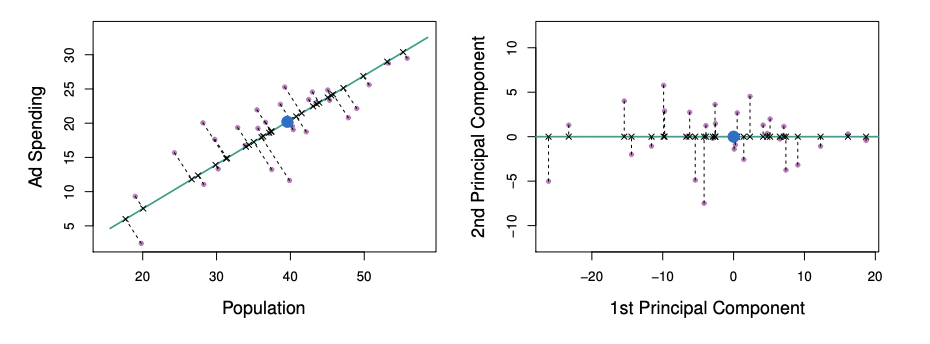
\includegraphics{pic/pca 2p.png}
    \caption{Left: our variables as axes; Right: Principle Components as axes}
    \label{fig:pca2}
\end{figure}

In the left plot, our first principle component ($PC_1$) is shown as the diagonal line. Additionally, we can see that this line has the most variance, i.e. if it was any other line, our points in the right plot would be more bunched together. Again, once we have decided our $PC_1$, $PC_2$ will be the line that has the next most uncorrelated variance, and this by construction is the orthogonal line.

\begin{note}
    by construction in the 2 variable case, we will only have 2 principle components and they will be orthogonal. This means that $PC_2$ will be perpendicular to the diagonal line in the left plot. This is why we can plot $PC_1$ against $PC_2$ in the right plot.
\end{note}

\begin{procedure}
    The first Principle Component, $v_i^1$, is a weighted average across $x_{i1}$ and $x_{i2}$ with the maximum variance across the $n$ observations. That is:

    \begin{equation}
        \underset{\varphi_1, \varphi_2}{\max}\underbrace{\sum_{i=1}^n (v_i^1)^2}_{\text{variance of PC1}} = \underset{\varphi_1, \varphi_2}{\max} \sum_{i=1}^n (\varphi_1 x_{i1} + \varphi_2 x_{i2})^2
    \end{equation}

    We constrain the maximisation problem with the following:
    \begin{equation*}
        \varphi_1^2 + \varphi_2^2 = 1
    \end{equation*}

    When choosing $\varphi_1, \varphi_2$ we are setting the direction in which we want to add variables, i.e. the rotation of the coordinate system.

    \begin{note}
        If we look back at Figure \ref{fig:pca2}, we can see that the transformation from the left plot to the right is the rotation of the coordinate system.
    \end{note}

    We then take out PC1, and work with the residualised data:

    \begin{equation*}
        \{\Tilde{x}_{i1}, \Tilde{x}_{i2}\}_{i=1}^n = \{x_{i1} - \varphi_1 v_{i1},x_{i2} - \varphi_2 v_{i1}\}_{i=1}^n
    \end{equation*}
    
\end{procedure}

\begin{example}
    When the maximum spread line is the 45 degree line, one can show that $\varphi_1 = \varphi_2 = \sqrt{1/2}$. That is:

    \begin{equation*}
        v_{i1} = \sqrt{\dfrac{1}{2}}(x_{i1} + x_{i2})
    \end{equation*}

    When we take out PC1, we are left with the residualised data:

    \begin{align*}
        \{\Tilde{x}_{i1}, \Tilde{x}_{i2}\}_{i=1}^n &= \{x_{i1} - \varphi_1 v_{i1},x_{i2} - \varphi_2 v_{i1}\}_{i=1}^n \\
        &= \{x_{i1} - \sqrt{\frac{1}{2}} v_{i1},x_{i2} - \sqrt{\frac{1}{2}} v_{i1}\}_{i=1}^n \\
        &= \left\{x_{i1} - \sqrt{\frac{1}{2}} \left(\sqrt{\frac{1}{2}}(x_{i1} + x_{i2})\right),x_{i2} - \sqrt{\frac{1}{2}} \left(\sqrt{\frac{1}{2}}(x_{i1}+x_{i2})\right)\right\}_{i=1}^n \\
         &= \left\{x_{i1} - \frac{1}{2}(x_{i1} + x_{i2}),x_{i2} - \frac{1}{2}(x_{i1}+x_{i2})\right\}_{i=1}^n \\
         &= \left\{\frac{1}{2}(x_{i1} + x_{i2}),\frac{1}{2}(x_{i2}-x_{i1})\right\}_{i=1}^n
    \end{align*}

    Then, our second principle component $v_{i2}$ is a weighted average of $\Tilde{x}_{i1}, \Tilde{x}_{i2}$, with the maximum residual variance across the $n$ observations. That is:

    \begin{equation}
        \underset{\varphi_1, \varphi_2}{\max}\underbrace{\sum_{i=1}^n (v_i^2)^2}_{\text{variance of PC2}} = \underset{\varphi_1, \varphi_2}{\max} \sum_{i=1}^n (\varphi_1 \Tilde{x}_{i1} + \varphi_2 \Tilde{x}_{i2})^2
    \end{equation}

    We find that when $\varphi_1 = \varphi_2 = \sqrt{\frac{1}{2}}$:
    \begin{align*}
    v_{i1} &= \sqrt{\frac{1}{2}}(x_{i1} + x_{i2}) \\
    v_{i2} &= \sqrt{\frac{1}{2}}(x_{i1} - x_{i2})
    \end{align*}
\end{example}

\subsubsection{Variance Accounting}

We will continue with the example in which $\varphi_1 = \varphi_2 = \sqrt{\frac{1}{2}}$. That is, the maximum variance line is the 45 degree line. We can find the variance of $v_{i1}$ and $v_{i2}$.

\begin{align*}
    \sum_{i=1}^n (v_{i1})^2 &= \frac{1}{2}\sum_{i=1}^n(x_{i1} + x_{i2})^2 = \frac{1}{2}\sum_{i=1}^n x_{i1} + \frac{1}{2}\sum_{i=1}^n x_{i2} + \sum_{i=1}^n x_{i1} x_{i2} \\
    \sum_{i=1}^n (v_{i2})^2 &= \frac{1}{2}\sum_{i=1}^n(x_{i1} + x_{i2})^2 = \frac{1}{2}\sum_{i=1}^n x_{i1} + \frac{1}{2}\sum_{i=1}^n x_{i2} - \sum_{i=1}^n x_{i1} x_{i2}
\end{align*}

\begin{shaded}
    Our observations:
    \begin{itemize}
        \item If $x_{i1}$ and $x_{i2}$ are correlated, the first principal component always has higher variance than the second.

        \item Together, the principal components explain all of the variance in $\{x_{i1}, x_{i2}\}_{i=1}^n$.
    \end{itemize}

    \hl{these observations generalise to factor models with $p$ variables.}
    
\end{shaded}

\subsubsection{General Model}

\begin{algo}

\begin{enumerate}
\hspace{1in}
    \item Set $\mathbf{\Tilde{X}^1 = X}$, an $n \times p$ matrix. Then for $k = 1, 2, \ldots, \min(n,p)$. 
    \item Find:
    \begin{equation}
        \varphi_k = \arg\underset{\varphi}{\max}\left\{\mathbb{V}ar\left(\mathbf{\Tilde{X}^1}\phi\right) = \mathbb{V}ar(v_{k1}, v_{k2}, \ldots, v_{kn})\right\}
    \end{equation}
    where $v_{ki} = \phi^\prime \mathbf{x}_i = \sum_{j=1}^px_{ij}\phi_{jk}$ and $\sum_{j=1}^p \phi_{jk}^2 = 1$
    \item Update rows of $\mathbf{\Tilde{X}^{k+1}}$ via $\mathbf{\Tilde{x}_i^k} - v_{ik} \times \varphi_k$
\end{enumerate}

\end{algo}

The PCA algo repeatedly fits both rotations and factors to minimise deviance across dimensions $j=1,2, \ldots, p$ and obs $i=1,2, \ldots, n$ for factor model

$$
\tilde{x}_{i j}^{k} \sim \mathcal{N}\left(v_{i k} \varphi_{j k}, \sigma_{k}^{2}\right)
$$
where $\tilde{x}_{i j}^{k}=\tilde{x}_{i j}^{k-1}-v_{i, k-1} \varphi_{k-1, j}$.

\begin{note}
    We haven't exactly described the algorithm, but we have described the intuition. In practice, the algo is minimising deviance.

$$
\sum_{j=1}^{p} \sum_{i=1}^{n}\left(x_{i j}-\sum_{k=1}^{K} \phi_{j k} v_{i k}\right)^{2}
$$
\end{note}

\subsubsection{Relationship between PCA and Factor Models}

The factor model interprets the data as

$$
\mathbb{E}\left(\mathbf{x}_{i}\right)=\varphi_{1} v_{i 1}+\varphi_{2} v_{i 2}+\ldots+\varphi_{K} v_{i K}=\Phi \mathbf{v}_{i} ; \quad i=1,2, \ldots, n
$$
Applying PCA we look for principal components such that

$$
v_{i k}=\varphi_{1 k} x_{i 1}+\varphi_{2 k} x_{i 2}+\ldots+\varphi_{p k} x_{i p}=\mathbf{x}_{i}^{\prime} \varphi_{k} ; \quad i=1,2, \ldots, n ; k=1,2, \ldots, K
$$

Stacking the $K$ PCs $\mathrm{PC}_{i}=\left(P C_{i 1}, P C_{i 2}, \ldots, P C_{i K}\right)$ implies

$$
\mathbf{P C}_{i}=\Phi^{\prime} \mathbf{x}_{i} ; \quad i=1,2, \ldots, n
$$

where $\Phi=\left(\varphi_{1}, \varphi_{2}, \ldots, \varphi_{K}\right)$ is a $p \times K$ matrix of PCA rotations.

By construction, the PCA rotation matrix is orthogonal $\Phi^{\prime} \Phi=\mathbf{I}$; hence,

$$
\Phi \mathrm{PC}_{i}=\Phi \Phi^{\prime} \mathbf{x}_{i}=\mathbf{x}_{i}
$$

so there is a factor model where factors are PCs from our PCA

\subsubsection{Number of PCs}

Unless the PCs are used for downstream prediction, it is difficult to cross-validate the number of PCs, $K$. People often look at \hl{the proportion of the total variance accounted for by a certain number of PCs}

\begin{align*}
    \text { Total Variance }=\sum_{j=1}^{p} \operatorname{Var}\left(x_{j}\right)&=\sum_{j=1}^{p} \frac{1}{n} \sum_{i=1}^{n} x_{i j}^{2} \\
    \text{Variance explained by the \textit{k}th PC, }\operatorname{Var}\left(P C_{i k}\right)&=\frac{1}{n} \sum_{i=1}^{n} PC_{i k}^{2} \\
    \text{Proportion of variance explained by \textit{K} PCs, }&=\frac{\sum_{k=1}^{K} \frac{1}{n} \sum_{i=1}^{n} P C_{i k}^{2}}{\sum_{j=1}^{p} \frac{1}{n} \sum_{i=1}^{n} x_{i j}^{2}}
\end{align*}

\newpage
\section{Experiments and Controls}

The aim of experiments is to find causal relationships between variables. This is much harder than just prediction. You need to make \textbf{"what if ..."} (counterfactual) predictions, and we will discuss ways of doing that.

\subsection{Potential Outcomes Framework}

Suppose the treatment $d$ is binary, i.e.

$$
d= \begin{cases}1 & \text { Treatment } \\ 0 & \text { No treatment }\end{cases}
$$

The outcome $y$ would depend on the treatment:

$$
y= \begin{cases}y(1) & \text { Treatment, } d=1 \\ y(0) & \text { No treatment. } d=0\end{cases}
$$

Meaning subject $i$ has the potential outcomes $\{y_i(1), y_i(0)\}$ and a treatment effect of $y_i(1) - y_i(0)$. The \hl{average treatment effect} (ATE) takes the expectation across subjects (i.e. the average)

$$
ATE \equiv \mathbb{E}[y(1)-y(0)]
$$

When we observe subject $i$'s outcome, they will either be treated or not: $y_i = y_i(1)$ or $y_i = y_i(0)$, but never both. We need an unobserved counterfactual:

\begin{itemize}
    \item $y_i(0)$ if $d_i = 1$: can be interpreted as the outcome of the treated subject $i$ if they had not been treated.
    \item $y_i(1)$ if $d_i = 0$: can be interpreted as the outcome of the non-treated subject $i$ had they been treated.
\end{itemize}

\begin{note}
    We can never get individual counterfactuals, but we can find the average counterfactual
\end{note}

\subsection{Randomised Controlled Trials}

\subsection{Conditional Ignorability}

\subsection{Linear Treatment Effect Model}

\subsection{LTE Lasso}



\appendix

\clearpage

\section{Dimension Reduction Methods}

\label{appendix: dimension reduction}

With our simple models, we look at controlling our variance by either using a subset of the original variables, or we shrink the coefficients towards zero i.e. using predictors $\mathbf{x_1, x_2, \ldots, x_p}$. \hl{Dimension reduction methods are a class of approach that transforms the predictors and then fits a least squares model using the transformed variables}.

\begin{definition}
    Let $Z_1, Z_2, \ldots, Z_M$ represent $M<p$ \textit{linear combinations} of our original $p$ predictors. 

    \begin{equation*}
        Z_m = \sum_{j=1}^p \phi_{jm}\mathbf{x_j}
    \end{equation*}

    for some constants $\phi_{1m}, \phi_{2m}, \ldots, \phi_{pm}$ for $m= 1, \ldots, M$. We can then fit the linear regression model:

    \begin{equation}
        \label{dim reduction lin reg}
        y_i = \theta_0 + \sum_{m=1}^M \theta_m z_{im} + \epsilon_i, \qquad i = 1, \ldots, n
    \end{equation}
    using least squares. All dimension reduction methods work in two steps:

    \begin{enumerate}
        \item Get the transformed predictors $Z_1, Z_2, \ldots, Z_M$.
        \item Fit the model with these $M$ predictors. 
    \end{enumerate}
    However, the choice of our new predictors (or equivalently the $\phi_{jm}$'s) can be achieved in different ways.
\end{definition}

\begin{note}
    Notice:

    \begin{equation*}
        \sum_{m=1}^M \theta_m z_{im} = \sum_{m=1}^M \theta_m \sum_{j=1}^p \phi_{jm}x_{ij} = \sum_{j=1}^p \sum_{m=1}^M \theta_m \phi_{jm} x_{ij} = \sum_{j=1}^p \beta_j x_{ij},
    \end{equation*}
    where
    \begin{equation*}
        \beta_j = \sum_{m=1}^M \theta_m \phi_{jm}.
    \end{equation*}
\end{note}

\subsection{Principal Component Analysis (PCA)}

PCA is a technique for reducing the dimension of an $n \times p$ data matrix $\mathbf{x}$. The \textit{first principal component} direction of the data is that along which the observations \textbf{vary the most} (more variance = more information = better regressor).

pg. 253 ISLR












\end{document}